%%%%%%%%%%%%%%%%%%%%%%%%%%%%%%%%%%%%%%%%%%%%%%%%%%%%%%%%%%%%%%%%%%%%%%%%

%%% LaTeX Template for AAMAS-2027 (based on sample-sigconf.tex)
%%% Prepared from the official AAMAS-2027 submission instructions.

%%%%%%%%%%%%%%%%%%%%%%%%%%%%%%%%%%%%%%%%%%%%%%%%%%%%%%%%%%%%%%%%%%%%%%%%

%%% Start your document with the \documentclass command.


%%% == IMPORTANT ==
%%% Use the first variant below for the final paper (including author information).
%%% Use the second variant below to anonymize your submission (no author information shown).
%%% For further information on anonymity and double-blind reviewing, 
%%% please consult the call for paper information
%%% https://warwick.ac.uk/fac/sci/dcs/aamas2027/calls/

%%%% For anonymized submission, use this
\documentclass[sigconf,anonymous]{aamas}

%%%% For camera-ready, use this. Switching back also means restoring the
%%%% acknowledgements near the end of this file.
%\documentclass[sigconf]{aamas}


%%% Load required packages here (note that many are included already).

\usepackage{balance} % for balancing columns on the final page
% placeins is loaded for the supplement's shared preamble habits only. Do not
% put \FloatBarrier between a result subsection and its full-width figure: a
% barrier there flushes the page early and leaves half of it blank, which is
% what it did before the figures were moved to the head of the subsection they
% belong to. Declaring a figure* at the head of its subsection places it at the
% top of the page the subsection runs onto, without a barrier.
\usepackage{placeins}

%%%%%%%%%%%%%%%%%%%%%%%%%%%%%%%%%%%%%%%%%%%%%%%%%%%%%%%%%%%%%%%%%%%%%%%%

%%% AAMAS-2027 copyright block (do not change!)

\makeatletter
\gdef\@copyrightpermission{
  \begin{minipage}{0.2\columnwidth}
   \href{https://creativecommons.org/licenses/by/4.0/}{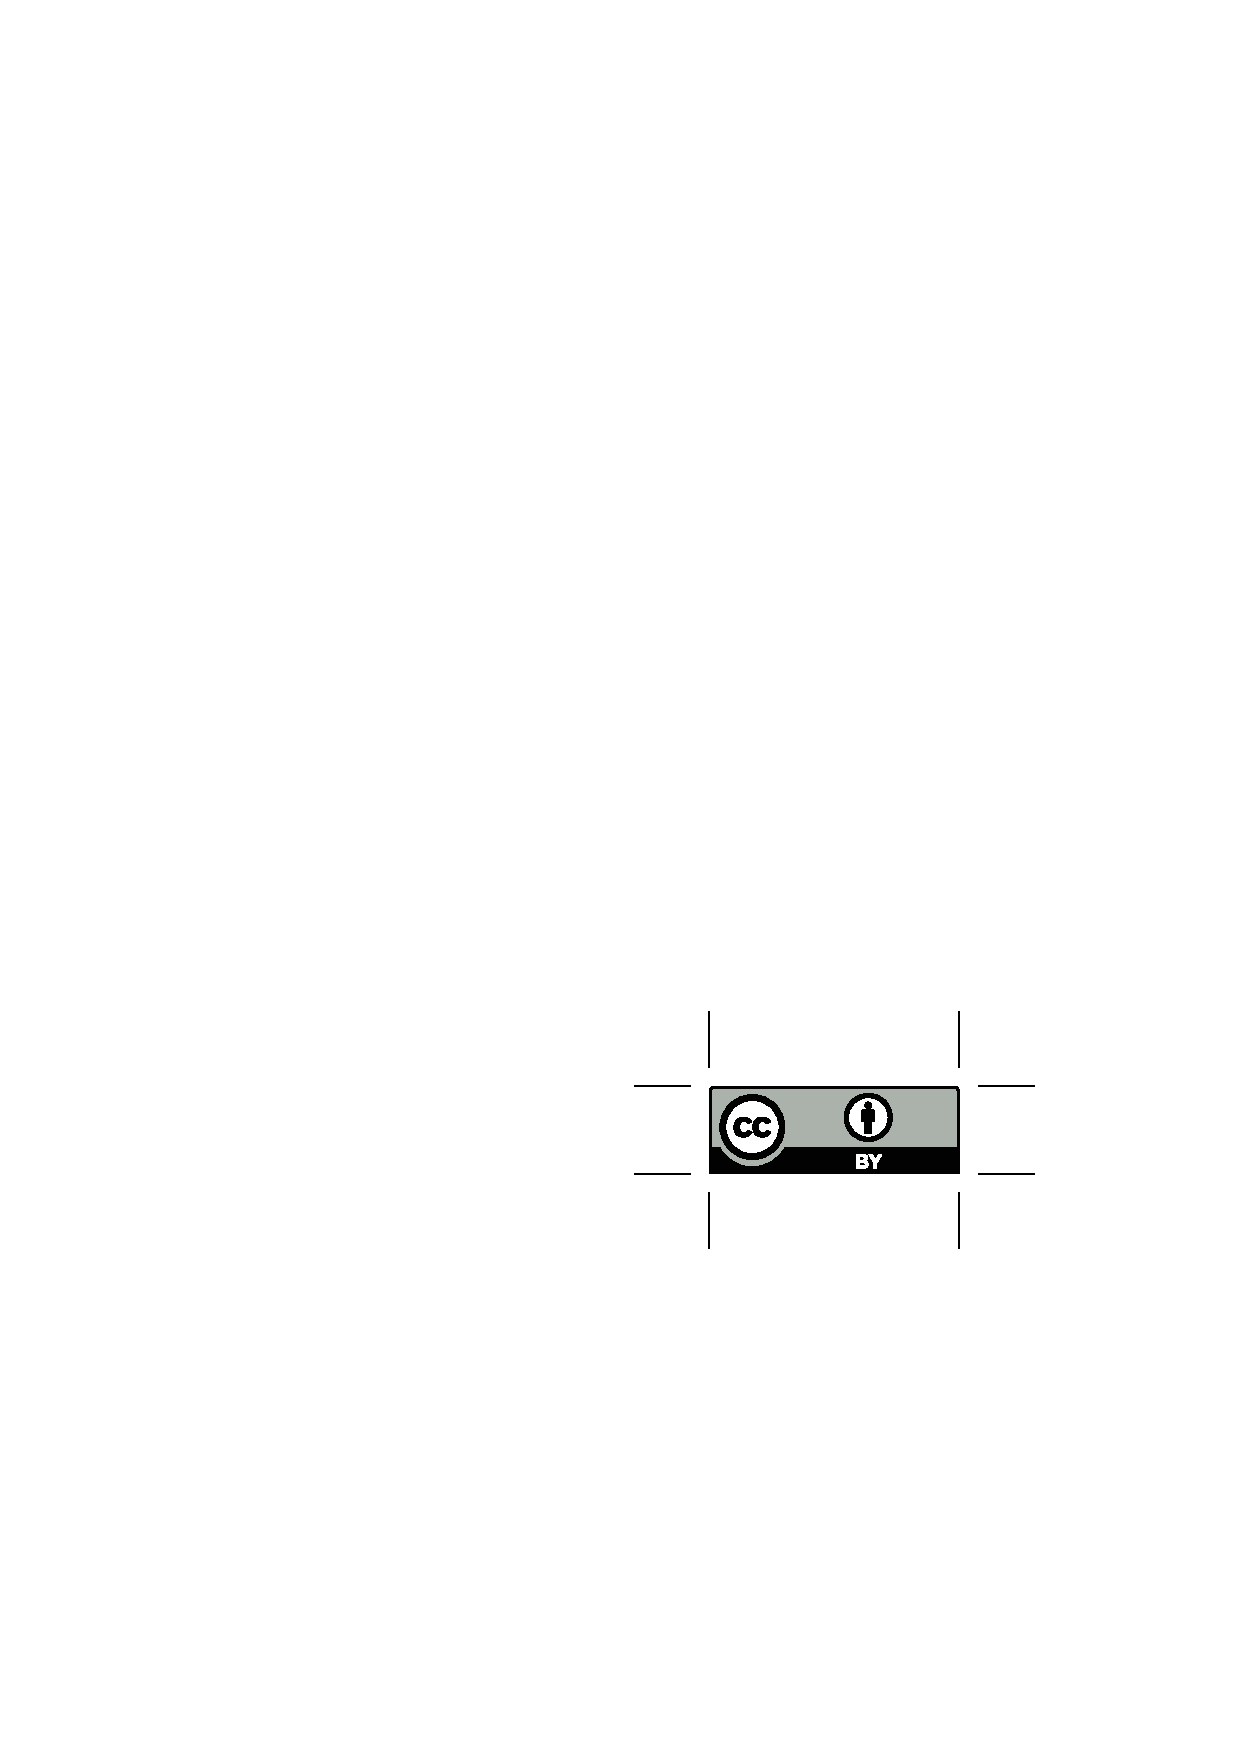
\includegraphics[width=0.90\textwidth]{by}}
  \end{minipage}\hfill
  \begin{minipage}{0.8\columnwidth}
   \href{https://creativecommons.org/licenses/by/4.0/}{This work is licensed under a Creative Commons Attribution International 4.0 License.}
  \end{minipage}
  \vspace{5pt}
}
\makeatother

\setcopyright{ifaamas}
\acmConference[AAMAS 2027]{Proc.\@ of the 26th International Conference
on Autonomous Agents and Multiagent Systems (AAMAS 2027)}{3--7 May 2027}{Hanoi, Vietnam}{M.~Baldoni, F.~Fang, W.~Yeoh, N.~Yorke-Smith (eds.)}
\copyrightyear{2027}
\acmYear{2027}
\acmDOI{}
%\acmPrice{}
\acmISBN{}


%%%%%%%%%%%%%%%%%%%%%%%%%%%%%%%%%%%%%%%%%%%%%%%%%%%%%%%%%%%%%%%%%%%%%%%%

%%%%%%%%%%%%%%%%%%%%%%%%%%%%%%%%%%%%%%%%%%%%%%%%%%%%%%%%%%%%%%%%%%%%%%%%

%%% Include any author-defined commands here.
         
\newcommand{\BibTeX}{\rm B\kern-.05em{\sc i\kern-.025em b}\kern-.08em\TeX}
\newcommand{\Safe}{\textsc{safe}}
\newcommand{\Unsafe}{\textsc{unsafe}}

%%%%%%%%%%%%%%%%%%%%%%%%%%%%%%%%%%%%%%%%%%%%%%%%%%%%%%%%%%%%%%%%%%%%%%%%

%%% == IMPORTANT ==
%%% Use this command to specify your submission number.
%%% In anonymous mode, it will be printed on the first page.

% Insert the assigned anonymous submission identifier after abstract registration.
% Leave empty in pre-registration builds so no placeholder appears in the PDF.
\newcommand{\SubmissionID}{}

\acmSubmissionID{\SubmissionID}

\submissionType{Research Paper Track}

%%% Use this command to specify the title of your paper.

%\title[]{LLM Agents Underrepresent Human Strategic Diversity in AI Development Races}
%\title[]{Humans Are More Diverse: Audited Frontier LLMs Show Extreme Policies in Idealised AI Development Races}

\title[]{More Than the Risk: Frontier LLM Behaviour in AI Development Races Depends on the Rival}

%%% Provide names, affiliations, and email addresses for all authors.
% \author{Nimue}
% \affiliation{
%   \institution{The Lady's Lake}
%   \city{Avalon}
%   \country{United Kingdom}}
% \email{lady.of.the.lake@avalon.uk}

% \author{Phu-Hoa Pham}
% \affiliation{
%   \institution{Vietnam National University of Ho Chi Minh City}
%   \institution{Ho Chi Minh City University of Science}
%   \city{Ho Chi Minh City}
%   \country{Vietnam}}
% \email{23122030@student.hcmus.edu.vn}
% \author{Phu-Quy Nguyen-Lam}
% \affiliation{
%   \institution{Vietnam National University of Ho Chi Minh City}
%   \institution{Ho Chi Minh City University of Science}
%   \city{Ho Chi Minh City}
%   \country{Vietnam}}
% \email{23122048@student.hcmus.edu.vn}
% \author{Dao Sy Duy Minh}
% \affiliation{
%   \institution{Vietnam National University of Ho Chi Minh City}
%   \institution{Ho Chi Minh City University of Science}
%   \city{Ho Chi Minh City}
%   \country{Vietnam}}
% \email{23122041@student.hcmus.edu.vn}
% \author{Trung-Kiet Huynh}
% \affiliation{
%   \institution{Vietnam National University of Ho Chi Minh City}
%   \institution{Ho Chi Minh City University of Science}
%   \city{Ho Chi Minh City}
%   \country{Vietnam}}
% \email{23122039@student.hcmus.edu.vn}
% \author{Chi-Nguyen Tran}
% \affiliation{
%   \institution{Vietnam National University of Ho Chi Minh City}
%   \institution{Ho Chi Minh City University of Science}
%   \city{Ho Chi Minh City}
%   \country{Vietnam}}
% \email{23122044@student.hcmus.edu.vn}

% \author{Minh-Trung Le}
% \affiliation{
%   \institution{Ho Chi Minh City University of Technology (HCMUT)}
%   \institution{Vietnam National University Ho Chi Minh City (VNUHCM)}
%   \city{Ho Chi Minh City}
%   \country{Vietnam}}
% \email{trung.leminh@hcmut.edu.vn}
% \author{Phong-Hao Le}
% \affiliation{
%   \institution{Ho Chi Minh City University of Technology (HCMUT)}
%   \institution{Vietnam National University Ho Chi Minh City (VNUHCM)}
%   \city{Ho Chi Minh City}
%   \country{Vietnam}}
% \email{hao.lephong@hcmut.edu.vn}

% \author{Dinh-Nam Nguyen}
% \affiliation{
%   \institution{Ho Chi Minh City University of Technology (HCMUT)}
%   \institution{Vietnam National University Ho Chi Minh City (VNUHCM)}
%   \city{Ho Chi Minh City}
%   \country{Vietnam}}
% \email{nam.nguyenkhmt@hcmut.edu.vn}
% \author{Thien-Ky Nguyen-Dong}
% \affiliation{
%   \institution{Ho Chi Minh City University of Technology (HCMUT)}
%   \institution{Vietnam National University Ho Chi Minh City (VNUHCM)}
%   \city{Ho Chi Minh City}
%   \country{Vietnam}}
% \email{ky.nguyendongthien@hcmut.edu.vn}

% \author{Elias Fern\'andez Domingos}
% \affiliation{
%   \institution{Vrije Universiteit Brussel}
%   \institution{Universit\'e Libre de Bruxelles}
%   \city{Brussels}
%   \country{Belgium}}
% \email{elias.fernandez.domingos@vub.be}

% \author{Le Hong Trang}
% \affiliation{
%   \institution{Ho Chi Minh City University of Technology (HCMUT)}
%   \institution{Vietnam National University Ho Chi Minh City (VNUHCM)}
%   \city{Ho Chi Minh City}
%   \country{Vietnam}}
% \email{lhtrang@hcmut.edu.vn}

% \author{The Anh Han}
% \affiliation{
%   \institution{School of Computing, Engineering and Digital Technologies}
%   \institution{Center for Digital Innovation,  Teesside University}
%   \city{Middlesbrough}
%   \country{United Kingdom}}
% \email{T.Han@tees.ac.uk}


% =========================================================
% Reusable affiliations
% =========================================================

\newcommand{\HCMUSaffiliation}{%
  \affiliation{%
    \institution{Ho Chi Minh City University of Science}
    \institution{Vietnam National University Ho Chi Minh City (VNU-HCM)}
    \city{Ho Chi Minh City}
    \country{Vietnam}
  }%
}

\newcommand{\HCMUTaffiliation}{%
  \affiliation{%
    \institution{Ho Chi Minh City University of Technology (HCMUT)}
    \institution{Vietnam National University Ho Chi Minh City (VNU-HCM)}
    \city{Ho Chi Minh City}
    \country{Vietnam}
  }%
}

\newcommand{\BrusselsAffiliation}{%
  \affiliation{%
    \institution{Vrije Universiteit Brussel}
    \institution{Universit\'e Libre de Bruxelles}
    \city{Brussels}
    \country{Belgium}
  }%
}

\newcommand{\TeessideAffiliation}{%
  \affiliation{%
    \institution{School of Computing, Engineering and Digital Technologies}
    \institution{Center for Digital Innovation, Teesside University}
    \city{Middlesbrough}
    \country{United Kingdom}
  }%
}

% =========================================================
% Equal-contribution authors, listed alphabetically
% =========================================================
\author{Phu-Hoa Pham}
%\authornotemark[1]
\HCMUSaffiliation
\email{23122030@student.hcmus.edu.vn}

\author{Duy-Minh Dao-Sy}
%\authornote{These authors contributed equally to this work.}
\HCMUSaffiliation
\email{23122041@student.hcmus.edu.vn}

\author{Trung-Kiet Huynh}
%\authornotemark[1]
\HCMUSaffiliation
\email{23122039@student.hcmus.edu.vn}

\author{Phu-Quy Nguyen-Lam}
%\authornotemark[1]
\HCMUSaffiliation
\email{23122048@student.hcmus.edu.vn}



\author{Chi-Nguyen Tran}
%\authornotemark[1]
\HCMUSaffiliation
\email{23122044@student.hcmus.edu.vn}
\author{Minh-Trung Le}
%\authornotemark[1]
\HCMUTaffiliation
\email{trung.leminh@hcmut.edu.vn}

\author{Phong-Hao Le}
%\authornotemark[1]
\HCMUTaffiliation
\email{hao.lephong@hcmut.edu.vn}

\author{Dinh-Nam Nguyen}
%\authornotemark[1]
\HCMUTaffiliation
\email{nam.nguyenkhmt@hcmut.edu.vn}

\author{Thien-Ky Nguyen-Dong}
%\authornotemark[1]
\HCMUTaffiliation
\email{ky.nguyendongthien@hcmut.edu.vn}



% =========================================================
% Corresponding authors, in the requested order
% =========================================================

\author{Elias Fern\'andez Domingos}
%\authornote{Corresponding authors.}
\BrusselsAffiliation
\email{elias.fernandez.domingos@vub.be}

\author{Le Hong Trang}
%\authornote{Corresponding authors.}
%\authornotemark[2]
\HCMUTaffiliation
\email{lhtrang@hcmut.edu.vn}

\author{The Anh Han}
%\authornotemark[2]
\TeessideAffiliation
\email{T.Han@tees.ac.uk}

%%% Use this environment to specify a short abstract for your paper.
\begin{abstract}
Large language models are increasingly used to advise and act on consequential
decisions. As such systems become more involved in organisational decision
making, an AI-safety question arises: how would frontier agents behave when
competition rewards speed while caution reduces catastrophic risk? We study this
question in an idealised AI-development race, where agents repeatedly choose
between slower safe development and faster unsafe development.

Across the tested eligible endpoints, risk responses share a qualitative direction
but differ in shape. Agents respond to increasing risk, with profiles ranging
from gradual adaptation to near-deterministic switching. Behaviour also depends
strongly on the opponent. In a scripted-rival study of five frontier-model
endpoints that passed a frozen task-validity screen,
changes in the rival's behaviour move the agents substantially, with a
magnitude that varies by endpoint and can overlap the effect of changing the
stated risk itself. Thus, self-play outcomes can reflect an interaction between
two copies of a policy rather than an intrinsic risk preference.

Eligible endpoints also show a distinctive relationship to the theoretical and
human benchmarks. An analysis extending the evolutionary comparison across the
eligible panel places the four graded profiles closer in response shape to the
weak-selection regime than to its strong-selection prediction, while
their action trajectories generally occupy a more concentrated observed
trajectory space than those of human participants: 13 of 15 eligible cells fall
below every draw of a dyad-matched human null. These results suggest that AI-mediated competitive
decisions may be model-specific, opponent-dependent and behaviourally
concentrated, motivating evaluation at the level of interactions and trajectories
rather than aggregate action rates alone. Claims are scoped to the tested endpoints,
one prompt version and one idealised game.
\end{abstract}

%%% Use this command to specify a few keywords describing your work.
%%% Keywords should be separated by commas.

% \keywords{Legends, Myths, Folktales}
\keywords{Large language models, AI development races, multi-agent systems, repeated games, AI safety, opponent-conditioned behaviour}

%%%%%%%%%%%%%%%%%%%%%%%%%%%%%%%%%%%%%%%%%%%%%%%%%%%%%%%%%%%%%%%%%%%%%%%%

%%% Include any author-defined commands here.
         
% \newcommand{\BibTeX}{\rm B\kern-.05em{\sc i\kern-.025em b}\kern-.08em\TeX}

%%%%%%%%%%%%%%%%%%%%%%%%%%%%%%%%%%%%%%%%%%%%%%%%%%%%%%%%%%%%%%%%%%%%%%%%
\begin{document}

%%% The following commands remove the headers in your paper. For final
%%% papers, these will be inserted during the pagination process.

%\pagestyle{fancy}
%\fancyhead{}

%%% The next command prints the information defined in the preamble.

\maketitle 

%%%%%%%%%%%%%%%%%%%%%%%%%%%%%%%%%%%%%%%%%%%%%%%%%%%%%%%%%%%%%%%%%%%%%%%%

\section{Introduction}
\label{sec:introduction}

LLMs are increasingly studied as agents for decision support and strategic
interaction \citep{herrStrategicBias2024,playing_repeated_games_with_llms}. As
organisations
consider delegating more strategic tasks to such systems, an AI-safety question
follows: if a decision about how fast and how carefully to develop a powerful
technology were delegated to a frontier model, what would the model decide, and
would its decision look like the ones people make? The question is prospective
throughout, and we do not claim that any organisation today hands a safety
decision to a language model. We claim only that the behaviour a model would
bring to such a decision is measurable now, in a controlled game. Controlled
evaluation before widespread deployment can expose interaction effects that
would be difficult to isolate in operational settings.

Competition over advanced artificial intelligence can create a safety
dilemma: each company may benefit from moving faster, but safety work slows it
down when rivals do not follow the same standard
\citep{ai_race_for_strategic_advantage,racing_to_the_precipice,role_of_Cooperation}.
An \emph{AI development race} is a simple game that represents this tension,
in which every player chooses each round between slower Safe development and
faster Unsafe development
\citep{to_regulate_or_not,artificial_intelligence_development_races}. The game
is idealised and does not model a real AI company in full. Its value is
control: it lets us hold the stated danger, the rival's behaviour and the
relative progress fixed one at a time, which no observation of real firms
allows. We reproduce the two-player game studied by
\citet{falling_behind_unsafe} and add a compatible multiplayer version based
on \citet{to_regulate_or_not}. We call one hosted model endpoint at one fixed
configuration an \emph{endpoint}; the same model family can be served under
different dated versions or provider settings.

Human experiments show why an average is the wrong thing to compare. In the
two-player study of \citet{falling_behind_unsafe}, the preregistered comparison
between the two higher private-risk conditions found no clear difference;
exploratory analyses instead linked later Unsafe choices to the opponent's
previous action, to whether the player was ahead or behind, and to the player's
first action, so an early choice changes the later path of the interaction. A
useful human and LLM comparison must therefore examine round-by-round
trajectories over the first five rounds, rather than only the overall Unsafe rate.

Two problems make that comparison harder than it looks. The first is that a
correctly formatted action is not an informed one. LLMs already play games of
this kind as simulated participants, decision-making agents and game-playing
systems
\citep{using_llm_to_simulate,out_of_one,playing_repeated_games_with_llms}, yet a
model can return a valid action without tracking the state, can predict an
opponent's pattern without acting on it
\citep{playing_repeated_games_with_llms}, and can distort one simulated
experiment while reproducing three others \citep{using_llm_to_simulate}; in a
repeated game a single such action changes the next state and every later round.
Neither a plausible trajectory nor a verbal strategy report is therefore
evidence here that the agent tracked the game, and an aggregate \Unsafe{} rate
close to the human one is not evidence that it reproduces human decision
dynamics or holds a general safety preference
\citep{synthetic_replacement_human}.

The second is that prompt-based evaluation is sensitive to presentation choices
that do not change what the task asks. Formatting, option order, response-token
identity, output-format requests, whitespace and persona all shift model output
\citep{sclarPromptFormatting2024,pezeshkpourOptionOrder2024,weiSelectionBias2024,salinasButterfly2024,zhengPersona2024},
and strategic choice is no exception: reversing action labels or reassigning
their payoffs changes choice frequencies \citep{herrStrategicBias2024},
decisions move with topic, actor and world framing
\citep{robinsonBurdenFraming2025}, and performance falls when a familiar default
mapping is replaced by a stated alternative \citep{wuCounterfactual2024}. We
therefore test wording, answer order, arithmetic disclosure, narrative framing
and opaque response codes separately, and do not treat one familiar presentation
as a neutral measuring instrument.

Reproducible game-based frameworks attack the same difficulty from the other
side. FAIRGAME standardises repeated-game experiments across models, languages
and persona conditions against game-theoretic predictions
\citep{buscemiFAIRGAME2025}; later work adds payoff scaling, a Public Goods Game
and supervised recognition of canonical strategies, and finds cooperation moving
opposite to its evolutionary benchmark
\citep{huynhUnderstanding2025,huynhPayoffScaling2026}. What those designs hold
constant is the opponent, because the opponent in them is another copy of the
model under test.

One more result shapes what a delegate population should be compared against.
Simulated populations recover broad contrasts while showing less heterogeneity
than the people they stand in for, in markets, survey populations and
persona-based simulation
\citep{delRioChanonaMarkets2025,synthetic_replacement_human,suhSurveyDistributions2025,wangHumanSubjectivity2024},
which is why position papers call social simulation defensible for exploratory
use until validated against the population of interest
\citep{anthisSocialSimulation2025}. Strategic-game evidence is similarly
unsettled, with policies that shift with parameters and framing, heuristics
applied more rigidly than people apply them, cooperation in place of the
predicted equilibrium, and action sequences that resist reproduction from
prompts alone
\citep{palCooperation2026,zhengBoundedRationality2025,yaoCompetition2026,luMultiTurn2026}.
A set of delegates that agrees with itself more than people do is a different
object from a delegate that is simply more or less cautious, so our human
comparison reports within-population diversity and not only aggregate
\Unsafe{} rates.

We therefore ask three questions about the delegate's behaviour.
\emph{Risk:} how do frontier agents trade speed against safety as the stated
chance of catastrophe rises? \emph{Rivalry:} are those choices a property of
the model, or do they emerge from the opponent the model happens to meet?
\emph{Humans and theory:} do the agents reproduce the strategic structure that
evolutionary game theory predicts, or the one human participants display?

Each answer changes how the next should be read. The four graded endpoints respond
gradually to the stated danger, while one endpoint replaces that trade-off with a
switch from always fast to always careful. But where we put the agent against
scripted code instead of a second copy of itself, the rival's stance shifts play
on every endpoint; its magnitude is endpoint-specific and can overlap the effect
of changing the stated danger. Neither external reference shows that shape: at
its usual strong-selection setting the evolutionary model predicts a switch
where the agents deliver a gradient, and
on raw first-five-round trajectories human participants use nearly the whole observed
trajectory space while eligible endpoints generally use a small part of it.

Three contributions follow. First, a scripted-rival design for repeated-game
evaluation and the critique it licenses. That an LLM's self-play behaviour need
not predict its behaviour against a different agent is known
\citep{lekeasNashSuppression2026}, and fixed opponents are
standard practice in this literature \citep{payneStrategicIntelligence2025};
what we add is the version that matters for a safety reading, that self-play
can hide the response to the treatment the study is about, measured against an
undisclosed rival whose policy is fixed by code. Second, a
population-level comparison with human participants read on first-five-round
trajectories rather than on aggregate rates, which is what makes the compression
of observed trajectories visible at all. Third, an auditable race mechanism in which the engine
and not generated text resolves every round, entered through a comprehension
screen that scores answers to frozen questions against ground truth and never
reads a race, so that the set of endpoints interpreted strategically was fixed by a
rule that cannot see the behaviour being interpreted. Exploratory multiplayer results remain in the
supplementary material, because the available position analysis covers two
checkpoints and cannot identify a general group-size effect.

Every behavioural conclusion is scoped to its tested endpoint, prompt version,
decoding contract, provider path and run period. The labels \Safe{} and
\Unsafe{} denote actions inside the experimental game and are not measurements
of general LLM safety, of a subjective risk preference, or of suitability for
autonomous deployment, and nothing measured here is a harm, a real safety
outcome, or an action taken by an organisation.

\section{Preliminaries}
\label{sec:preliminaries}

We first specify the two-player game reproduced from \citet{falling_behind_unsafe} (\S\ref{sec:prelim-2p}). We additionally evaluate an exploratory $N$-player extension; its mechanism and results are reported in the supplementary material. Figure~\ref{fig:mechanism} summarises the two-player instrument and the three empirical lenses used in the main results.

% This overview keeps the game mechanism visible while putting the delegation
% question and the three behavioural lenses first.

\begin{figure*}[t]
  \centering
  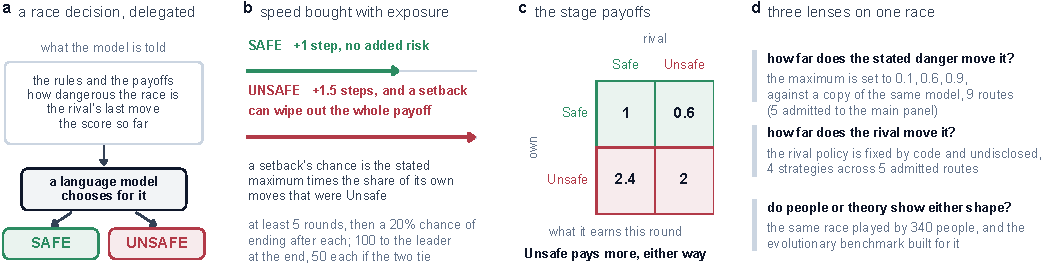
\includegraphics[width=\textwidth]{../figures/paper/delegation_overview.pdf}
  \caption{The game and the questions it lets us ask. (a) The model receives
  the rules, stated danger, rival's last move and current score, then returns
  either \Safe{} or \Unsafe{}. (b) \Safe{} advances one step without added
  risk; \Unsafe{} advances faster but raises the chance that the winner's
  payoff is wiped out. (c) The two-player stage-payoff matrix makes \Unsafe{}
  attractive against either rival move, so the delayed terminal risk supplies
  the safety tension. (d) The main results examine stated-risk response,
  scripted-rival response, and comparison with human trajectories and the
  evolutionary benchmark.}
  \label{fig:mechanism}
  \Description{Four-panel overview of the AI development race. Panel a shows
  the information given to a language model and its Safe or Unsafe decision.
  Panel b shows the speed gained by Unsafe and the delayed private setback
  risk, together with the hidden horizon and terminal prize. Panel c shows the
  two-by-two stage-payoff matrix with own action as rows and rival action as
  columns. Panel d lists the three empirical lenses: stated danger, scripted
  rival, and the human and evolutionary references.}
\end{figure*}


\subsection{Two-player game}
\label{sec:prelim-2p}

Two companies $i \in \{1,2\}$ play a repeated race. In every round $t$, both simultaneously choose an action $a_i^t \in \{S, U\}$ (Safe, Unsafe) and commit to it before either learns the other's choice, and only then does the round resolve (Figure~\ref{fig:mechanism}a). Resolution has two parts. First, progress accumulates as $P_i^t = P_i^{t-1}+\sigma(a_i^t)$ with $\sigma(S)=1.0$ and $\sigma(U)=1.5$, so Unsafe always closes the race faster. Second, the round pays a stage payoff $\pi_i^t=\pi(a_i^t,a_{-i}^t)$, read off the fixed matrix (own action by row, opponent action by column, Figure~\ref{fig:mechanism}b):
\begin{equation}
    \pi = \begin{pmatrix} 1.0 & 0.6 \\ 2.4 & 2.0 \end{pmatrix}.
    \label{eq:2p-matrix}
\end{equation}
Unsafe strictly dominates Safe at the stage level (row 2 exceeds row 1 in both columns): the only cost of Unsafe development enters later, through accumulated private risk.

The race lasts a minimum of $5$ rounds; after every completed round from round $5$ onward it terminates with probability $0.2$, giving an expected horizon $\mathbb{E}[T]=9$. Neither company is ever told the horizon, so neither can condition on the current round being the last (Figure~\ref{fig:mechanism}a). Termination resolves in two further steps. First, the company with the higher cumulative progress $P_i^T$ wins a prize $B=100$, split $50/50$ on an exact tie. Second, and only for that winner or tied winners, an accumulated private setback risk is drawn:
\begin{equation}
    q_i(T) = p_r^{\max} \cdot \frac{n_i^U(T)}{T}, q_i(T) \in [0,1], p_r^{\max}\in\{0.10,0.60,0.90\},
    \label{eq:risk}
\end{equation}
where $n_i^U(T)$ counts company $i$'s Unsafe choices over the whole race and $p_r^{\max}$ is a treatment-level constant, assigned once per race, that we vary across three risk levels. If the draw against $q_i(T)$ fails, that company's entire race payoff, accumulated stage payoffs plus the prize, is zeroed. A company that ends behind is never subject to the draw: it keeps its stage payoffs regardless of how much Unsafe it played, but receives no share of the prize (Figure~\ref{fig:mechanism}a). This asymmetry, in which risk is built by both companies but realised only against whoever is ahead, is what makes Unsafe development a genuine gamble rather than a free speed advantage.

\subsection{Game-theoretic benchmark}
\label{sec:theory-benchmark}

\begin{table}[t]
\caption{The four benchmark strategies. Each is fixed by its opening move and
by what it does afterwards, so AS and AU never react to the other player while
CS and CAS react to nothing else. These four are also the fixed rivals of
\S\ref{sec:results-scripted}.}
\label{tab:benchmark-strategies}
\centering
\footnotesize
\begin{tabular}{@{}llp{0.34\linewidth}@{}}
\toprule
Strategy & Opening & Every later round \\
\midrule
Always Safe (AS) & \Safe{} & \Safe{} \\
Conditionally Safe (CS) & \Safe{} & copy the rival's last move \\
Conditionally Antisocial Safe (CAS) & \Unsafe{} & copy the rival's last move \\
Always Unsafe (AU) & \Unsafe{} & \Unsafe{} \\
\bottomrule
\end{tabular}
\end{table}


The two incentives oppose each other. Stage-level dominance rewards Unsafe
immediately, while across the full race Unsafe choices raise the setback risk
for a winner or tied winner, so the best action can depend on the risk
condition, earlier actions, and the expected response of other players.

We use four simple strategies as a theory benchmark, defined in
Table~\ref{tab:benchmark-strategies}. Two of them ignore the other player and
two of them do nothing but answer it, which is what makes the set a benchmark:
it separates a fixed disposition from a reaction. In the reconstructed finite-population evolutionary model of
\citet{falling_behind_unsafe}, the most common strategy changes from AU at
$p_r^{\max}=0.10$, to CAS at $0.60$, and to CS at $0.90$: the theory predicts
not one fixed amount of Unsafe play but a risk-dependent shift between
unconditional speed, an aggressive opening and conditional restraint. We use
this as a qualitative benchmark, not as a fitted model of LLM output, because
prompted self-play trajectories are not samples from an evolutionary
population.

\section{Experimental design and evidence policy}
\label{sec:design}
\subsection{Agent protocol and units of analysis}

At each decision an agent receives a versioned prompt carrying the round, the assigned maximum private risk, the disclosed state, and the preceding revealed action profile when $t>1$. Same-round decisions are sealed: every response comes from the same pre-action snapshot, before the engine resolves actions, progress, payoffs and risk, so the environment rather than generated text determines all transitions. Raw response, parsed action, retry and parser status, pre-turn state, terminal record, configuration and seed allocation are retained for every decision.

Sampling parameters here are provider-visible contracts, not intended
settings. The run manifests record a requested temperature of 0.7 that the
hosted SDK forwarded on no baseline endpoint, and no provider confirmed an
effective value. Seed handling was endpoint-specific: the SDK stripped the
requested seed on the Google endpoints and forwarded it, application
unconfirmed, on the OpenAI and Anthropic ones.

Both seats of a race are the same endpoint, so every gameplay rate below is
mirror-match play, until \S\ref{sec:results-scripted} fixes the rival instead.

The main behavioural outcome is whether an agent chooses Unsafe. The race,
not the individual decision, is the main independent experimental unit,
because decisions from one race depend on earlier states and are not
separate random samples; uncertainty is grouped by race or matched repetition
wherever possible. A cell's rate pools its decisions, while a paired contrast
is the mean over matched repetitions of the within-repetition difference in
race-level rates, so each repetition counts once however long its race ran;
the two therefore need not differ by exactly the printed contrast. A \emph{parse failure} is a response that does not follow
the required action format, and because the fallback action changes later
states, one marks the whole race as contaminated.
\subsection{Evidence strata and admission}

We separate confirmatory gameplay from diagnostic presentation checks. A
\emph{diagnostic pilot} is an exploratory test for possible effects or failures;
it does not estimate a stable effect. A \emph{confirmatory} study tests a
question under a plan fixed before any result is inspected, with its protocol,
endpoint, prompt, configuration, race count and exclusion rules recorded in the
run manifest. We never pool the two strata.

One presentation check is confirmatory and is described in the supplementary
material: on two endpoints, a fully crossed rerun retells the same game under a
race story or as an abstract contest, and substitutes the opaque response
codes $P$ and $Q$ for \Safe{} and \Unsafe{} under both code mappings. A
task-validity screen gates which endpoints enter the behavioural comparison. It
is an inclusion rule, not a behavioural outcome, and all gameplay results
below are analysed without ranking endpoints by its scores.

\subsection{Quality-control screen on the endpoints}
\label{sec:design-screen}

An action that parses is not evidence that the agent followed the race. Before
behavioural analysis, each endpoint therefore answered the same frozen bank of 20
probes over six task-validity domains, three times. An endpoint entered the study
only if it cleared the fixed thresholds of 80\% overall accuracy, 75\% state
reconstruction and 75\% terminal scoring. Five of nine endpoints passed; the
other four still played the same confirmatory baseline and remain available
throughout the trajectory-diversity analyses for transparency and sensitivity
checks.

The screen reads probes and never reads a race, so gameplay cannot change its
verdict. Two eligible endpoints pass one screening domain at the minimum attainable
score. We therefore use the screen only as a task-validity
inclusion rule, never as a capability axis or a behavioural contrast. Full
screening results are retained in the supplementary material, and whether such
a screen measures comprehension at all is the subject of a concurrent
submission \citep{anonConcurrentScreen2026}; no result below rests on a
screen score.

\section{Results}
\label{sec:results}

These endpoints respond to the danger they are told about, and their behaviour
also depends strongly on the rival. Four eligible endpoints have profiles closer
in response shape to the weak-selection evolutionary benchmark; Claude Opus 5 is
the step-like exception. Eligible endpoints generally occupy a more concentrated
observed trajectory space than human participants do: 13 of 15 endpoint-risk cells fall
below every draw of the primary dyad-matched human null. The four subsections
take those results in turn. A screen-failing endpoint appears below only where it
is named as excluded. Three- to five-player
races, full model tables, predictive diagnostics and robustness checks are in
the supplementary material.

\subsection{How agents trade speed against safety}
\label{sec:results-risk}

There is a shared directional response across the eligible endpoints. \Unsafe{}
play is non-increasing with the stated maximum private risk on every eligible
endpoint, while the shape varies: four of the five give ground gradually and the
fifth switches (Figure~\ref{fig:risk-response}). Each endpoint supplied 30 races
and 558 dependent within-race decisions under one frozen protocol, with zero
parse failures and ten races per risk cell. Risk contrasts use matched repetition
blocks, and race-weighted reanalysis preserves the non-increasing response on
every eligible endpoint (supplementary material).

\begin{figure}[t]
    \centering
    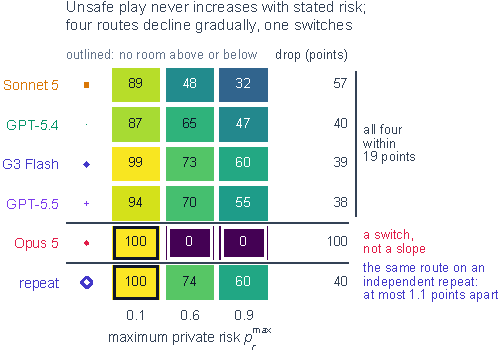
\includegraphics[width=\columnwidth]{../figures/paper/risk_response.pdf}
    \caption{\Unsafe{} play is non-increasing with stated risk. The four graded
    endpoints fall within a 19-point band; Claude Opus 5 switches from the ceiling
    to the floor. The outlined cells are at a
    boundary and therefore leave no room for a larger or smaller observed
    rate. The repeat row is the same Gemini 3 Flash endpoint collected under an
    independent administration.}
    \label{fig:risk-response}
    \Description{Heatmap of Unsafe play for five eligible endpoints across three
    maximum private-risk conditions, with a right-hand column showing the drop
    from the lowest to the highest condition. Four graded endpoints lie in a
    narrow band and Claude Opus 5 forms a separate switch row; an additional
    repeat row is shown below.}
\end{figure}

The four graded endpoints, spanning three providers, have risk-response drops within
a 19-point band, from 38.2 to 57.0 percentage points. We report that band
rather than an average over all five, because averaging a switch with four
slopes returns 54.8 points, a figure no graded endpoint is near and which one row
produces.

That fifth endpoint follows a threshold-like policy. Claude Opus 5 plays \Unsafe{}
on all 186 decisions at risk $0.1$ and \Safe{} on all 372 decisions above it,
with no race inside a cell departing from that. Its 100-point figure reaches
the largest value on the scale, and because no risk level was run between
$0.1$ and $0.6$, the location of its transition is not measured.

At the highest risk the game offers, where a winner's whole payoff is zeroed
with probability up to $0.9$ in proportion to how much \Unsafe{} it played, the
four graded endpoints still play \Unsafe{} on roughly a third to three fifths of
their decisions against a copy of themselves, in the $r{=}0.9$ column of
Figure~\ref{fig:risk-response}. This variation shows that risk-aware behaviour
remains contingent on endpoint and interaction context. Two endpoints
can also reach a similar rate through very different sets of races, which
\S\ref{sec:results-diversity} measures directly.

For the repeated Gemini 3 Flash endpoint, the profile was stable across two
administrations. Repeating the whole protocol on that endpoint under the same frozen
contract moved no risk cell by more than 1.1 points over 186 decisions, against
a 93.0-point spread in risk response across the nine endpoints, and moved its own
risk response from 38.7 to 40.3. This bounds run-to-run variation for that endpoint
at this sample size; it licenses no such bound for an endpoint collected once, which
matters here because no provider confirmed applying the requested sampling seed.

Representation-equivalent prompt changes also move rates. The directional risk
response survives a fully crossed narrative-by-symbol rerun on two endpoints,
although swapping the opaque action-code mapping shifts \Unsafe{} play by
8.3--9.5 percentage points (see the supplementary material).


\begin{figure*}[t]
  \centering
  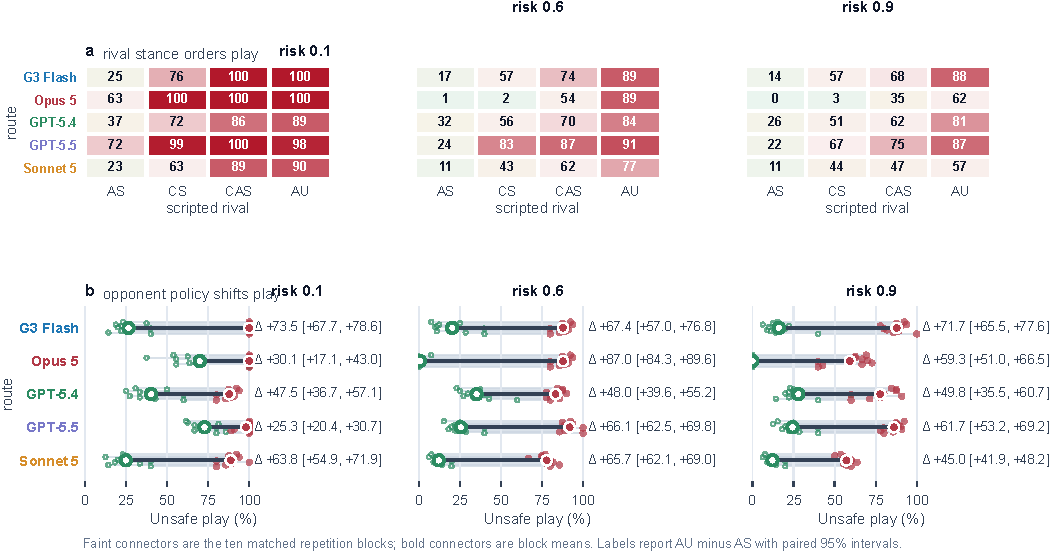
\includegraphics[width=\textwidth]{../figures/paper/scripted_opponent_main.pdf}
  \caption{A shared opponent policy changes an endpoint's play. Panel (a) is a
  response surface: each tile is an eligible endpoint's Unsafe rate under one
  scripted opponent, with columns ordered from Always Safe to Always Unsafe and
  facets for the three maximum-risk conditions. Panel (b) shows the empirical
  response to changing only the opponent policy: open points are the Always
  Safe opponent and filled points are the Always Unsafe opponent, with faint
  matched repetition blocks behind each bold mean connector. Labels report the
  paired Always-Unsafe minus Always-Safe contrast with 95\% intervals.
  Within-endpoint contrasts are the estimands; cross-endpoint magnitudes are
  descriptive under heterogeneous contracts.}
  \Description{Two-panel figure. Panel a contains three response matrices,
  one per risk level, with five endpoint rows and four ordered scripted-opponent
  columns; every tile prints the measured Unsafe rate. Panel b contains three
  risk facets with the same five endpoint rows. Open and filled points show the
  Always Safe and Always Unsafe opponent rates, faint connectors show the ten
  matched repetition blocks, bold connectors show their means, and right-side
  labels give paired 95 percent intervals.}
  \label{fig:scripted-opponent-main}
\end{figure*}

\subsection{The rival substantially reshapes play}
\label{sec:results-scripted}

\begin{table*}[t]
\caption{What moves play: the rival's stance against the stated danger, on the
five eligible endpoints. The rival columns give the paired Always Unsafe minus
Always Safe contrast at one stated danger. The danger columns give the paired
risk $0.1$ minus risk $0.9$ contrast with the rival held at one policy. Every
entry is in percentage points of \Unsafe{} play with a 95\% interval over the
same ten matched repetition blocks, so columns are comparable within an
endpoint. Cross-endpoint magnitudes are descriptive, because decoding contracts
differ across endpoints.}
\label{tab:risk-versus-rival}
\centering
\footnotesize
\begin{tabular}{@{}lrrrrr@{}}
\toprule
& \multicolumn{3}{c}{Rival stance, at a fixed stated danger} & \multicolumn{2}{c}{Stated danger, against a fixed rival} \\
\cmidrule(lr){2-4}\cmidrule(l){5-6}
Endpoint & at $0.1$ & at $0.6$ & at $0.9$ & safe rival & unsafe rival \\
\midrule
Gemini 3 Flash   & 73.5 [67.8, 78.7] & 67.4 [57.1, 76.6] & 71.7 [65.6, 77.5] & 10.4 [5.4, 15.7] & 12.2 [8.2, 16.1] \\
GPT-5.4          & 47.5 [37.0, 57.2] & 48.0 [40.0, 55.0] & 49.8 [35.8, 60.5] & 12.3 [6.2, 18.6] & 10.0 [5.9, 14.2] \\
GPT-5.5          & 25.3 [20.3, 30.6] & 66.1 [62.5, 69.9] & 61.7 [53.5, 69.1] & 48.3 [43.1, 54.3] & 11.9 [8.4, 15.2] \\
Claude Sonnet 5  & 63.8 [54.8, 72.1] & 65.7 [62.2, 68.9] & 45.0 [42.0, 48.2] & 12.7 [8.5, 16.6] & 31.5 [27.2, 35.3] \\
Claude Opus 5    & 30.1 [16.5, 42.8] & 87.0 [84.3, 89.6] & 59.3 [51.2, 66.5] & 69.9 [57.1, 83.5] & 40.7 [33.5, 48.7] \\
\bottomrule
\end{tabular}
\end{table*}


In the five endpoints tested against scripted rivals, the observed behaviour does
not support a context-independent risk profile. Across these endpoints, changing
who is on the other side moves play substantially, but the magnitude varies by
endpoint and can overlap the effect of changing how dangerous the race is told to
be. Every rate reported so far is mirror-match play, in which
the rival is the endpoint. One campaign fixes the rival instead.

The rival in that campaign is code, not a model. Five eligible endpoints each
played the four benchmark strategies of \S\ref{sec:theory-benchmark} at all
three risk levels: 60 cells, ten races each, 600 races and 5{,}580 endpoint
decisions with no parse failure anywhere. It is never disclosed to the endpoint,
and every one of its 5{,}580 recorded rival moves was
recomputed afterwards from the endpoint's own recorded history, which no cell
failed. The endpoint's seat is counterbalanced five and five inside each cell, and
each contrast is taken inside a repetition, so the hidden horizon is differenced
out. Because rival-policy assignment is fixed and exogenous within matched
blocks, the direction of a difference between rival policies is identified.
Conditional policies can still respond mechanically to the endpoint's previous
move, as specified by the fixed policy.

Coverage is complete across the five endpoints, but decoding contracts are not
homogeneous across endpoints. Cross-endpoint differences in effect magnitude are
therefore descriptive rather than controlled endpoint comparisons; the full
contract provenance is reported in the supplement.

Table~\ref{tab:risk-versus-rival} puts the two candidate drivers of play on the
same endpoints and the same matched blocks. Changing the rival while the stated
danger is held fixed moves play by at least a quarter of an endpoint's decisions
in every one of the fifteen cells. Changing the stated danger while the rival is
held safe moves play by about ten points on three endpoints and by half or more
of their decisions on the other two. Neither effect dominates the other, because
the largest risk contrast is larger than the smallest rival contrast and the two
ranges overlap. What the table establishes is that the rival is never the small
term, not that it is always the large one, and which of the two is larger is a
property of the endpoint rather than of the game.

All five tested endpoints respond to the scripted opponent policy. \Unsafe{} play
rises from the rival that always plays \Safe{}, through the two conditional
rivals, to the rival that never plays \Safe{}, in fourteen of fifteen
endpoint-by-risk cells, with strict ordering in twelve. The one reversal is
GPT-5.5 at risk $0.1$, where the CAS rival draws $100.0\%$ and
Always Unsafe is $97.8\%$, so this is a boundary case rather than a clean
counterexample (Figure~\ref{fig:scripted-opponent-main}a). The paired
difference between the two unconditional rivals is
positive in every cell. All fifteen paired-block 95\% intervals have positive
lower bounds, with the smallest at $+16.5$ points
(Figure~\ref{fig:scripted-opponent-main}b). The response to the stated risk
survives the change of design as well: against a fixed safe rival, no endpoint's
\Unsafe{} rate rises as the stated risk rises.

How strongly an endpoint answers its rival is itself endpoint-specific, and
Table~\ref{tab:risk-versus-rival} separates two behaviours rather than two sizes
of one behaviour. Gemini 3 Flash and GPT-5.4 answer the rival by about the same
amount whatever the stated danger, so for them the rival and the danger are
separate inputs. The other three answer it far more strongly once the danger is
real than when it is negligible, so for them the rival is what the danger is read
through. The level differs as well as the swing: against a rival that never
plays \Unsafe{}, GPT-5.4 still does so about a third of the time at every stated
danger, which no other endpoint does. These are separate endpoint samples, so
intervals that fail to overlap are a conservative sign of a difference rather
than a test of one.

A mirror-match rate is therefore an interaction outcome of one policy meeting
itself, rather than a stand-alone measurement of how an endpoint treats risk.
Self-play exceeds the fixed-safe rate in thirteen of fifteen cells; the two
exceptions are Claude Opus 5 at the floor, lower at risk $0.6$ ($0.0\%$ against
$1.1\%$) and tied at $0.0\%$ at risk $0.9$. On Gemini 3 Flash at the lowest risk, the distance is a
lower bound because nine of its ten mirror-match races have every decision
\Unsafe{}. These results motivate treating mirror-match rates as interaction
outcomes rather than endpoint-level risk preferences.

The bound on the finding is the design itself. Four reduced strategies are four
points in a space of policies rather than a sample of rivals, so this
establishes what an endpoint does against \emph{these} rivals, on one game and one
prompt version, and five commercial endpoints are not a sample from a
population of models.



\begin{figure*}[t]
    \centering
    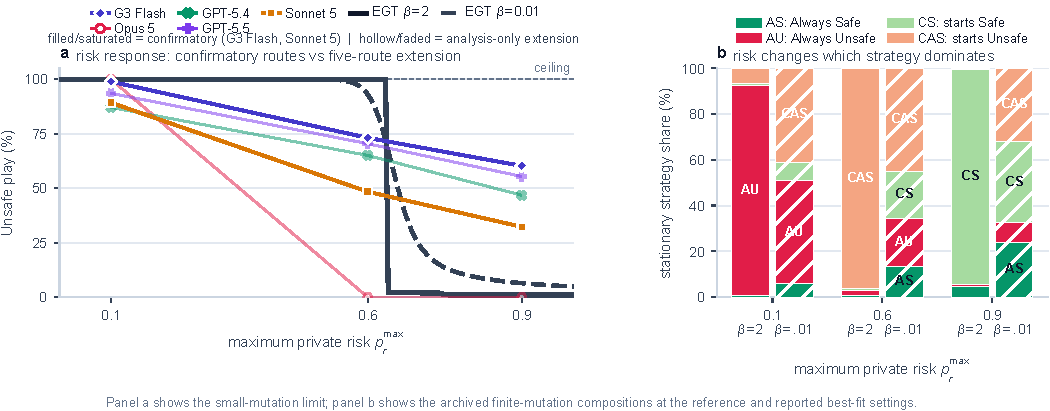
\includegraphics[width=\textwidth]{../figures/paper/theory_versus_behaviour.pdf}
    \caption{The evolutionary benchmark and the eligible endpoint profiles in
    a common risk coordinate. (a) The direct comparison keeps the two
    prespecified profiles, Gemini 3 Flash and Claude Sonnet 5, with individual
    race rates behind their means. The small-mutation limit is step-like at
    strong selection and graded near weak selection, while both direct profiles
    move gradually. (b) Each dumbbell compares the canonical RMSE over the
    three matched risk levels for the reference strong-selection regime
    ($\beta=2,\ \mu=.02$) and the reported best weak-selection regime
    ($\beta=.01,\ \mu=.05$). All five eligible endpoints are closer to the
    weak-selection fit; Claude Opus 5 remains the qualitative near-step
    exception in panel (a).}
    \label{fig:theory-behaviour}
    \Description{Two-panel comparison. Panel a plots Unsafe play against maximum
    private risk for the reconstructed evolutionary model at strong and weak
    selection, with individual race rates and means for Gemini 3 Flash and
    Claude Sonnet 5. Panel b is a five-row dumbbell plot comparing each eligible
    endpoint's RMSE under the reference strong-selection regime and its best
    weak-selection fit over the three observed risk levels.}
\end{figure*}

\subsection{Weak selection better matches the graded response shape}
\label{sec:results-theory}

The four graded endpoint profiles are closer to the source study's human-fitted
weak-selection regime than to its strong-selection reference setting
(Figure~\ref{fig:theory-behaviour}b). The direct profiles remain the clearest
shape comparison: Gemini 3 Flash gives 98.9\%, 73.1\% and 60.2\%, and Claude
Sonnet 5 gives 89.2\%, 48.4\% and 32.3\% over 30 races each. At the reference
setting of \citet{falling_behind_unsafe}, $\beta=2$ and $\mu=\beta/Z$ lose 98
points inside a risk step of $0.005$ (Figure~\ref{fig:theory-behaviour}a).
The all-five fit shows that Claude Opus 5 is the qualitative exception: its
profile is near-step rather than graded, even though its weak-selection RMSE is
still lower than its reference RMSE.

In the evolutionary benchmark, the abrupt transition arises under strong
selection and becomes graded under weak selection. We swept
selection strength across $\beta \in [0.001, 10]$ crossed with three mutation
rules, 90 stationary-distribution cells, each estimated from independent chains
with the between-chain spread retained so that a badly mixed cell cannot be
mistaken for a result. As $\beta$ falls towards neutrality the predicted
high-risk \Unsafe{} rate rises off the floor and the model's own risk response
becomes graded, which is the shape the endpoints show. At $\beta=0.01$ with
$\mu=0.05$ the model predicts 87.3\%, 63.9\% and 38.0\%, the closest cell in the
entire sweep to both direct endpoints, within 9.6 percentage points of Claude Sonnet 5
and 15.4 of Gemini 3 Flash in root-mean-square error.

The weak-selection cell is not one we chose to fit: $\beta=0.01$ and
$\mu=0.05$ are the values the source study reports as its own best fit to human
play. The interpretation stays bounded. A stationary distribution
describes strategy frequencies in a population under selection and mutation,
while our measurements are prompted decisions in self-play; the agreement in
shape says the graded risk response is consistent with weak selection and
high exploration, not that the endpoints are evolving. What the sweep
establishes is narrower and still useful: a claim that LLM agents contradict the
evolutionary benchmark cannot rest on one setting of the selection strength,
because the sign of the high-risk gap depends on it.



\subsection{Eligible endpoints exhibit lower trajectory diversity than humans}
\label{sec:results-diversity}

Twenty people asked to run this race do not behave alike; twenty copies of a
frontier endpoint very nearly do. Human participants arrive at their average level
of \Unsafe{} play through many different histories, while each eligible endpoint
reuses a small set of them, so an endpoint can match the human mean without
resembling the human population at all. We measure this on first-five-round
trajectories. Each player contributes one exact paired trajectory, a ten-bit
string read within its own risk condition; because the progress increments are
fixed, that string fully specifies the first-five-round joint-action trajectory.
The comparison covers all nine endpoints that faced the screen, eligible and
excluded alike, on the confirmatory baseline, 60
trajectories per endpoint, against 340 complete human trajectories from the
de-identified dataset of \citet{falling_behind_unsafe}. That single published
study of a single game is the only human reference here, which bounds every
human comparison below to that population and that mechanism.

Of 341 released participants, 340 provide complete first-five-round trajectories
and 338 provide complete dynamic-model records. Among the complete trajectories,
168 source dyads contribute 336 trajectories; four complete trajectories have no
complete partner after de-identification and are not used in the dyad null.
Before using this dataset as an external reference, we validated the
reconstruction by refitting the source
study's published dynamic specification on its released data: 2{,}888
participant-round observations from 338 participants in 172 race-pair clusters
(see the supplementary material).

Figure~\ref{fig:diversity} counts distinct first-five-round trajectories in
matched samples of twenty, against $20{,}000$ human resamples of ten complete
dyads at each risk. The human sample is larger, so matching prevents sample
size from inflating its diversity, while dyad sampling preserves the unit of
interaction. Eighteen of 27 endpoint cells, including 13 of the 15 eligible cells,
fall below every dyad draw. The participant-level sensitivity gives 21 of 27,
including all 15 eligible cells; the primary dyad-null floors are 12, 15 and 13
distinct trajectories at risks $0.1$, $0.6$ and $0.9$. The complementary
participant-level table records effective counts of 18.9, 19.7 and 19.3 and
mean pairwise distances of 0.47, 0.50 and 0.50. Panel b sorts the observed paths
by frequency and panel c displays the modal five-round joint-action sequence.
The same cells support two numerical checks reported in the supplement: Hill
$q{=}1$ counts effective trajectories and mean pairwise Hamming distance measures
separation of their ten action bits. Under that complementary Hill $q{=}1$
analysis, every eligible endpoint sits entirely below the human interval at every
risk level.

The concentration is strongest for Claude Opus 5, which produces a single
trajectory, repeated by all 20 of its trajectories, at every risk level, while
Claude Sonnet 5 uses two at risk $0.1$. Concentration is also distinct from
level: Gemini 3 Flash and GPT-5.5 finish within five points of each other at the
highest risk and use a similar number of distinct trajectories, 12 and 13, yet the
Gemini trajectories sit half again as far apart from one another, 0.41 against 0.27
in mean pairwise distance.

Under the participant-level sensitivity, two endpoints are the only
exceptions, and the screen refuses both of them.
GPT-5.4 mini uses 20, 17 and 17 distinct trajectories out of 20 at
risks $0.1$, $0.6$ and $0.9$, and GPT-5.4 nano 16, 19 and 16; both land inside
the participant-level human null at every risk level, and no other endpoint reaches
it once under that sensitivity. On this measure they are not less diverse than
people. Under the primary dyad null, GPT-5.4 and GPT-5.5 also meet the finite-draw
floor at risk $0.9$, so the cluster-aware headline is 13 of 15 eligible cells
rather than all 15. Because the two exceptions are outside the eligible set
fixed by the inclusion rule of \S\ref{sec:design-screen} before any race was
read, they are reported, not interpreted as strategic diversity.

\begin{figure}[!b]
    \centering
    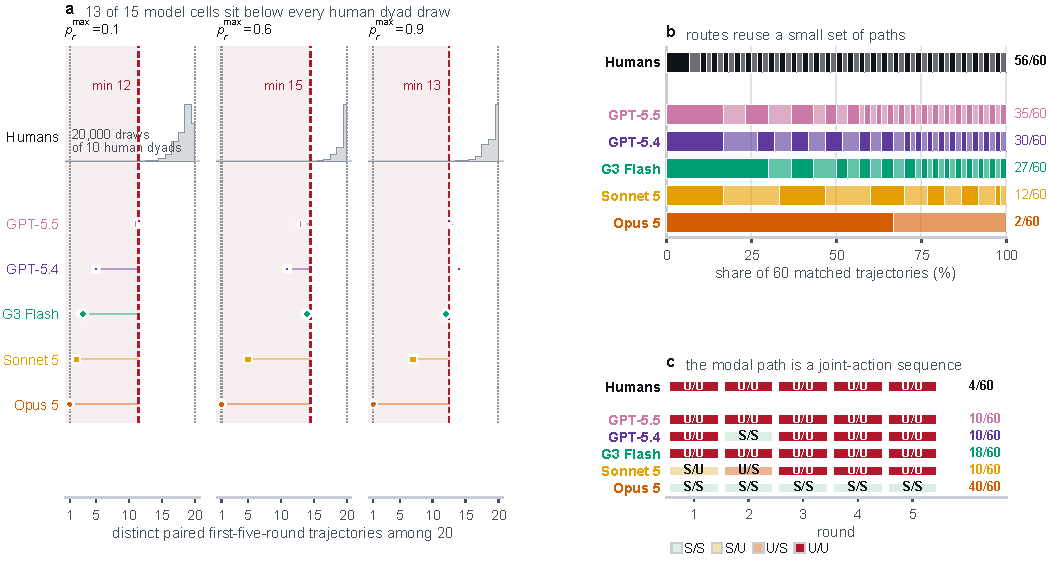
\includegraphics[width=\columnwidth]{../figures/paper/human_versus_model.pdf}
    \caption{Human participants occupy a broader observed trajectory space than
    most eligible endpoint-risk cells under a dyad-clustered null. Panel a compares
    distinct paired first-five-round trajectories with $20{,}000$ draws of ten
    complete human dyads; 13 of 15 eligible cells fall below every dyad draw.
    The participant-level null is a sensitivity analysis and places all 15 below
    every draw. Panel b sorts the 60
    matched trajectories by path frequency; panel c shows the modal pooled
    joint-action path. Each tile is the focal endpoint's action followed by its
    rival's.}
    \label{fig:diversity}
    \Description{Panel a shows three facets, one per risk condition, each with a
    histogram of a human dyad-resampling null and one marker per checkpoint placed
    on the same axis, with the shaded region marking counts no human dyad draw reached.
    Panel b shows frequency-sorted composition bars for the 60 matched
    trajectories. Panel c shows the modal five-round joint-action path for each
    population as one tile per round.}
\end{figure}

The same picture holds one level down, on the rates themselves. Raw
player-level \Unsafe{} rates, plotted per risk condition in the supplementary
material, spread across nearly the whole available range for humans at every
risk level while each checkpoint occupies a narrow band of its own. Similarity
between a checkpoint's aggregate \Unsafe{} rate and the human mean therefore
does not imply that it reproduces the human distribution. A two-dimensional
embedding of the same space is in the supplementary material; we rest no
conclusion on it, because recolouring the same coordinates by outcome separates
them almost entirely by \Unsafe{} rate.

Populations that look alike in rate can still be following different observed
rules. Exploratory classifier and feature analyses in the supplement suggest
that possibility, but use earlier pilot rosters containing neither GPT-5.4
nor GPT-5.5, so they support no claim about the eligible panel.

\section{Discussion and conclusion}
\label{sec:discussion}

These agents incorporate both the stated risk and the rival's stance. \Unsafe{}
play is non-increasing as the stated chance of catastrophe rises on every
eligible endpoint, while on the five endpoints where the rival was replaced by scripted
code, the rival's stance changes behaviour substantially, with a magnitude that
varies by endpoint and can overlap the effect of changing risk. In this game, the
five tested endpoints are therefore
strongly context-sensitive: how the other side behaves can be more informative
than the risk level alone.

Two things follow for how an agent of this kind should be measured. The first
is that a rate collected in self-play carries the rival inside it, so it cannot
be quoted as the endpoint's own disposition, and a design that wants the
disposition has to fix the rival by code and audit the moves that rival actually
made. The second is that an aggregate rate is not a description of a population
of agents. Twenty copies of an endpoint reach their average through far fewer
distinct histories than twenty people do, so two systems can report the same
headline rate while one of them has effectively one way of playing the game and
the other has twenty. A safety argument that rests on a matched average is
therefore resting on the weakest of the available comparisons.

The human experiment is an external behavioural reference, not a target an
agent should reproduce. Where an endpoint matches a human association, the two
populations behave similarly on that one measured aspect of this task; it
does not follow that they share a mechanism, and a mismatch does not
invalidate the human result.

Four limitations bound the claims directly. Nine commercial endpoints are not a
sample from a population of models, and any two of them differ in far more than
the one property a comparison names, so every contrast drawn between endpoints in
this paper is descriptive and none of it separates an endpoint's behaviour from its
provider, its scale or its training. The scripted-rival campaign covers five
    endpoints and four reduced strategies, which are four points in a space of
policies rather than a sample of rivals. The human comparison rests on one
published study of one game, 340 complete trajectories, and we do not add a
second human dataset, because any other dataset would change the game as well
as the population. And the evolutionary comparison is a reconstruction audited
against pinned EGTtools source \citep{fernandezDomingos2020Egttools} rather
than a bitwise reproduction of
undisclosed author code, so it bounds the regime in which the benchmark is read
rather than fitting the agents.

Four further limits are worth stating. The crossed presentation design covers
two endpoints, enough to show the effect replicates but not to characterise
endpoints in general. A matched group-size grid exists on one
endpoint, but adding a company changes the stage payoff and the prompt length too,
so no pure group-size effect is identifiable. Sampling was not under our
control: no provider confirmed the requested temperature, and the seed was
stripped on the Google endpoints and forwarded unconfirmed on the others. And this
game models a private speed-versus-safety trade-off and nothing else, with no
collective harm, regulation, communication or uncertainty about real
capabilities.

Each of these limits points somewhere specific. The rival was fixed by code
here because a fixed rival is what makes the contrast identifiable, and the
natural next step is a rival that is itself an agent with a declared and audited
policy, which would test whether the response survives against something that
can adapt. The population result was read on one game, and reading it on a
second game with the same trajectory measure would show whether the compression
travels with the agent or with the task. And because the stated danger and the
rival are separate inputs on two endpoints and not on the other three, an
experiment that varies both together on more endpoints would say whether that
split is a stable property of an endpoint or an artefact of the three danger
levels this game offers.

Code, the de-identified run records and a checker that recomputes every
reported quantity from them are provided with the supplementary material and
will be released publicly with the final version.

% Acknowledgements name individuals, their institutions and a grant number, so
% they identify the authors. The class does not suppress this section in
% anonymous mode, it prints whatever is here. Restore the block below for the
% camera-ready, together with the non-anonymous \documentclass at the top.
%
% \section*{Acknowledgements}
% T.A.H. acknowledges travel and accommodation support from the Ho Chi Minh City University of Technology (HCMUT), VNUHCM (Adjunct Professorship scheme HCMUT\text{-}VNUHCM). L.H.T acknowledges the Ho Chi Minh City University of Technology (HCMUT), VNUHCM for supporting this study.
% TAH is supported by EPSRC (grant EP/Y00857X/1).
 
\clearpage
\bibliographystyle{ACM-Reference-Format}
% \bibliography{sample}
\bibliography{references}


%%%%%%%%%%%%%%%%%%%%%%%%%%%%%%%%%%%%%%%%%%%%%%%%%%%%%%%%%%%%%%%%%%%%%%%%

\end{document}
